\section{E1: fitting the training set}
\label{sec:e1}
Every tree in Table~\ref{tab:e1} is a depth-3 tree (7 routers, 8 leaves) with router width 32 and leaf width 128, trained with the mixture loss, batch size 256, and stopped as soon as training accuracy reached 100\%. All ten runs reached 100\% training accuracy, in 10 to 125 epochs (Figure~\ref{fig:e1}), with no data augmentation and no regularisation other than the small balance term. Hard routing keeps 100\% training accuracy in every case and changes test accuracy by at most 0.5 points, so the routers end up nearly deterministic even though they were trained soft.

\begin{table}[!htbp]
\centering\small
\begin{tabular}{llrrrrrr}
\toprule
dataset & features & params & per image & epochs & train acc & test acc & test acc (hard) \\
\midrule
CIFAR-10 & random, shared & 1290k & 231k & 75 & 100.0 & 59.4 & 59.1 \\
CIFAR-10 & cnn, shared & 411k & 73k & 45 & 100.0 & 85.0 & 84.9 \\
CIFAR-10 & cnn, matched & 288k & 41k & 125 & 100.0 & 84.8 & 84.7 \\
CIFAR-10 & resnet, shared & 1210k & 217k & 20 & 100.0 & 82.5 & 82.1 \\
CIFAR-10 & resnet, matched & 841k & 118k & 30 & 100.0 & 81.1 & 80.7 \\
\midrule
Cats vs Dogs & random, shared & 1281k & 230k & 70 & 100.0 & 73.6 & 73.6 \\
Cats vs Dogs & cnn, shared & 403k & 72k & 75 & 100.0 & 91.7 & 91.6 \\
Cats vs Dogs & cnn, matched & 280k & 39k & 120 & 100.0 & 91.5 & 91.4 \\
Cats vs Dogs & resnet, shared & 1202k & 216k & 10 & 100.0 & 90.6 & 90.6 \\
Cats vs Dogs & resnet, matched & 833k & 117k & 20 & 100.0 & 90.7 & 90.3 \\
\bottomrule
\end{tabular}

\caption{E1. ``per image'' counts the parameters evaluated under hard routing (3 routers and 1 leaf). Test accuracy is with soft routing unless marked hard.}
\label{tab:e1}
\end{table}

\begin{figure}[!htbp]
\centering
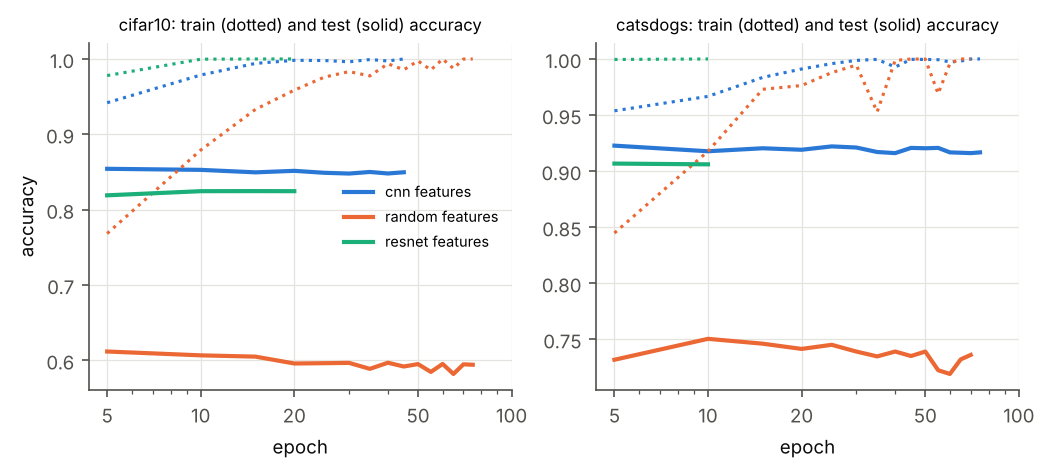
\includegraphics[width=0.92\linewidth]{e1_curves.png}
\caption{E1 training (dotted) and test (solid) accuracy, shared features. Training accuracy reaches 1.0 for every trunk; test accuracy is fixed early and is set by the trunk.}
\label{fig:e1}
\end{figure}

What the table says:
\begin{itemize}
\item \emph{Test accuracy is set by the features.} Random features give 59\% (CIFAR-10) and 74\% (Cats vs Dogs); ImageNet ResNet-18 features give 82\% and 91\%; the CNN trained on the task gives 85\% and 92\%. The tree memorises the training set equally well on all three.
\item \emph{The tree adds nothing on top of a good trunk.} The CNN trunk's own linear head scores 85.8\% (CIFAR-10) and 92.4\% (Cats vs Dogs) on the test set, slightly above the tree trained on its features (85.0\% and 91.7\%). E4 shows the same for ResNet features: a linear classifier matches the 1.2M-parameter tree.
\item \emph{Matched features cost little.} Feeding routers only the shallow ResNet stages (192 numbers instead of 960) cuts the parameters used per image from 217k to 118k and loses 1.3 points on CIFAR-10 and nothing on Cats vs Dogs. With the CNN trunk (routers read 64 shallow features) the per-image count falls from 73k to 41k for a loss of 0.2 points on both datasets. Routers do not need deep features to pick a branch.
\end{itemize}

\section{E3: receptive fields of the nodes}
\label{sec:rf}
For every router of the E1 trees (shared features, ResNet and CNN trunks) we measured:
\begin{enumerate}
\item which classes it sends left and right (test images, hard routing), and the normalised mutual information (NMI) between its decision and the class;
\item its most confident images on each side;
\item its \emph{effective receptive field} \cite{luo2016}: the mean over 64 images that reach the node of $|\partial g_j/\partial x|$, summed over colour channels, with gradients taken through the frozen trunk back to the pixels. The \emph{saliency radius} is the saliency-weighted mean distance from the image centre in units of the half-width; a uniform map gives 0.765 and a map concentrated at the centre gives 0;
\item an image synthesised to push the router hardest each way (gradient ascent on the router score from a grey image, with jitter and a total-variation penalty).
\end{enumerate}
The same saliency is computed for each leaf's score of the true class. We also trained a \emph{pixel tree} (linear routers directly on standardised pixels, leaves with 64 hidden units), whose router weight vectors can be drawn as images. Figures~\ref{fig:rf-cd}--\ref{fig:pixel} show the nodes; Table~\ref{tab:e3sum} summarises them and Tables~\ref{tab:e3-c10}--\ref{tab:e3-cd} list the ResNet routers.

\begin{figure}[p]
\centering
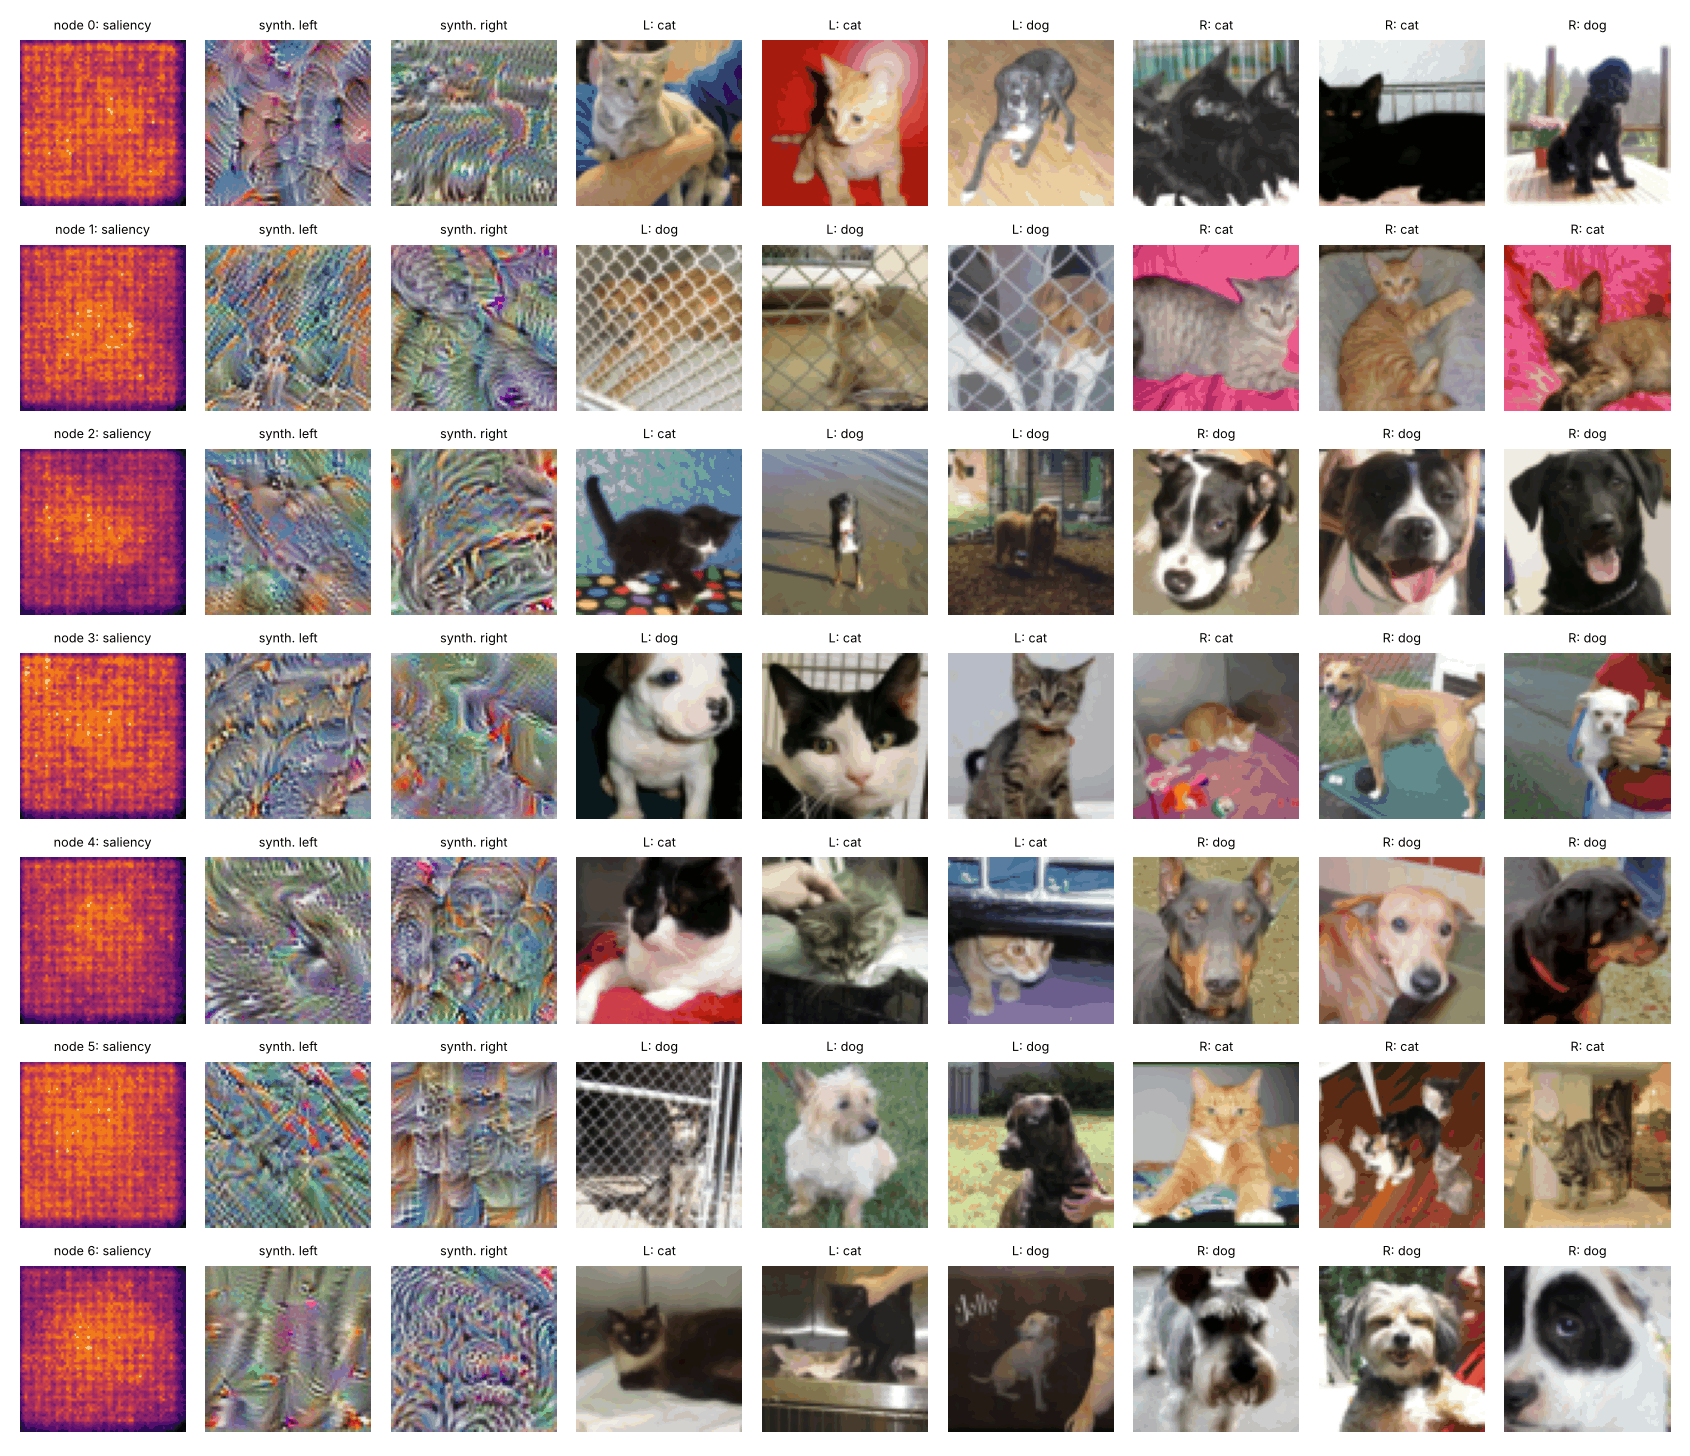
\includegraphics[width=\linewidth]{e3_routers_catsdogs_resnet.png}
\caption{Cats vs Dogs, ResNet features: the 7 routers (rows). Columns: mean input-gradient saliency over images reaching the node; synthesised images pushing the router left and right; the 3 most confident left images; the 3 most confident right images. Node 1 separates dogs behind wire fences and in cages from cats on pink and soft blankets; node 0 sends dark animals right; node 2 separates full-body shots on the ground from close-up dog faces.}
\label{fig:rf-cd}
\end{figure}

\begin{figure}[p]
\centering
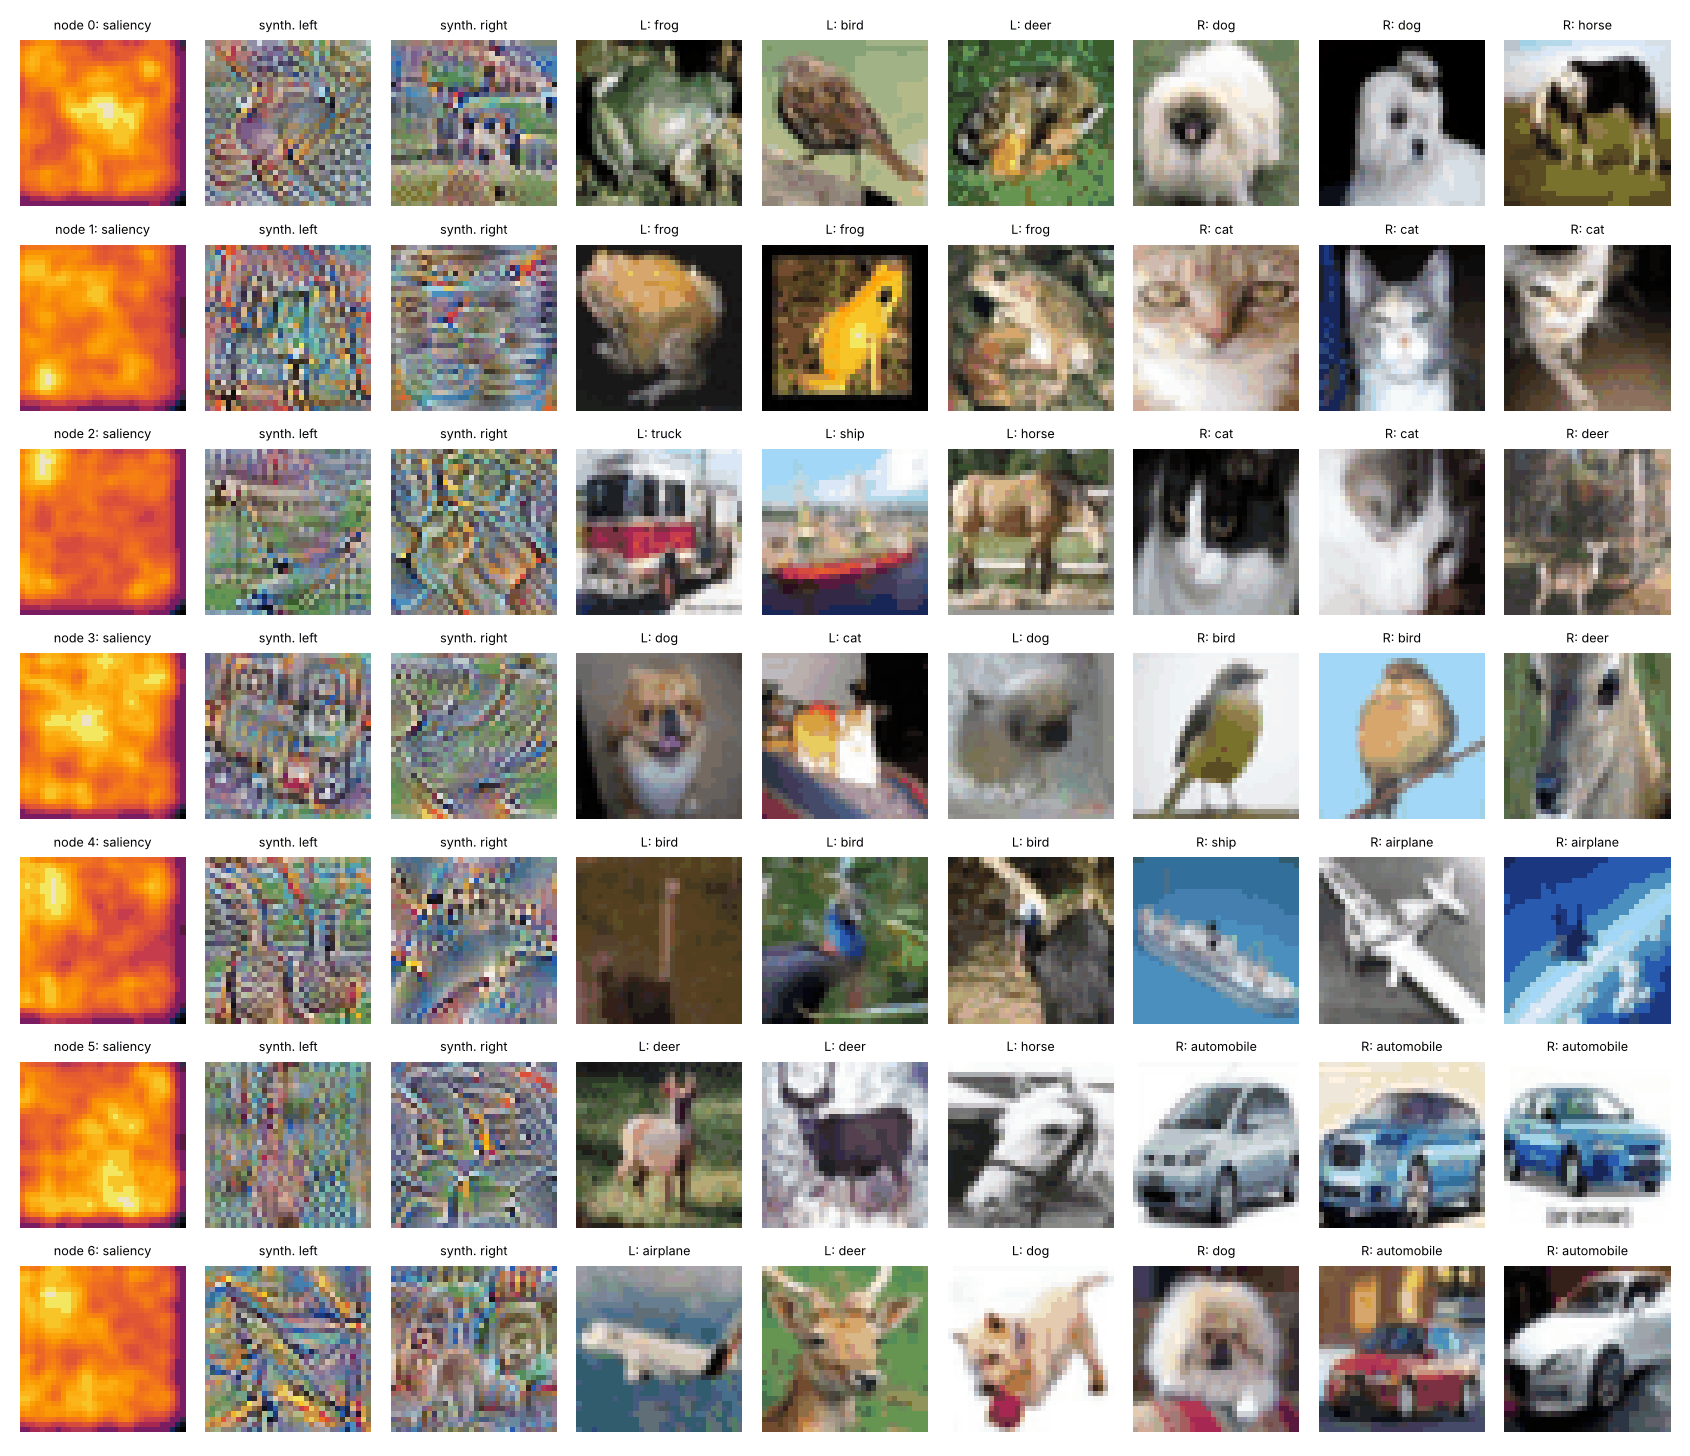
\includegraphics[width=\linewidth]{e3_routers_cifar10_resnet.png}
\caption{CIFAR-10, ResNet (ImageNet) features, same layout. Saliency is spread over the whole image and the synthesised images are textures. Node 4 sends birds in foliage left and ships and aeroplanes on blue backgrounds right; node 5 sends deer and horses left and cars right.}
\label{fig:rf-c10}
\end{figure}

\begin{figure}[p]
\centering
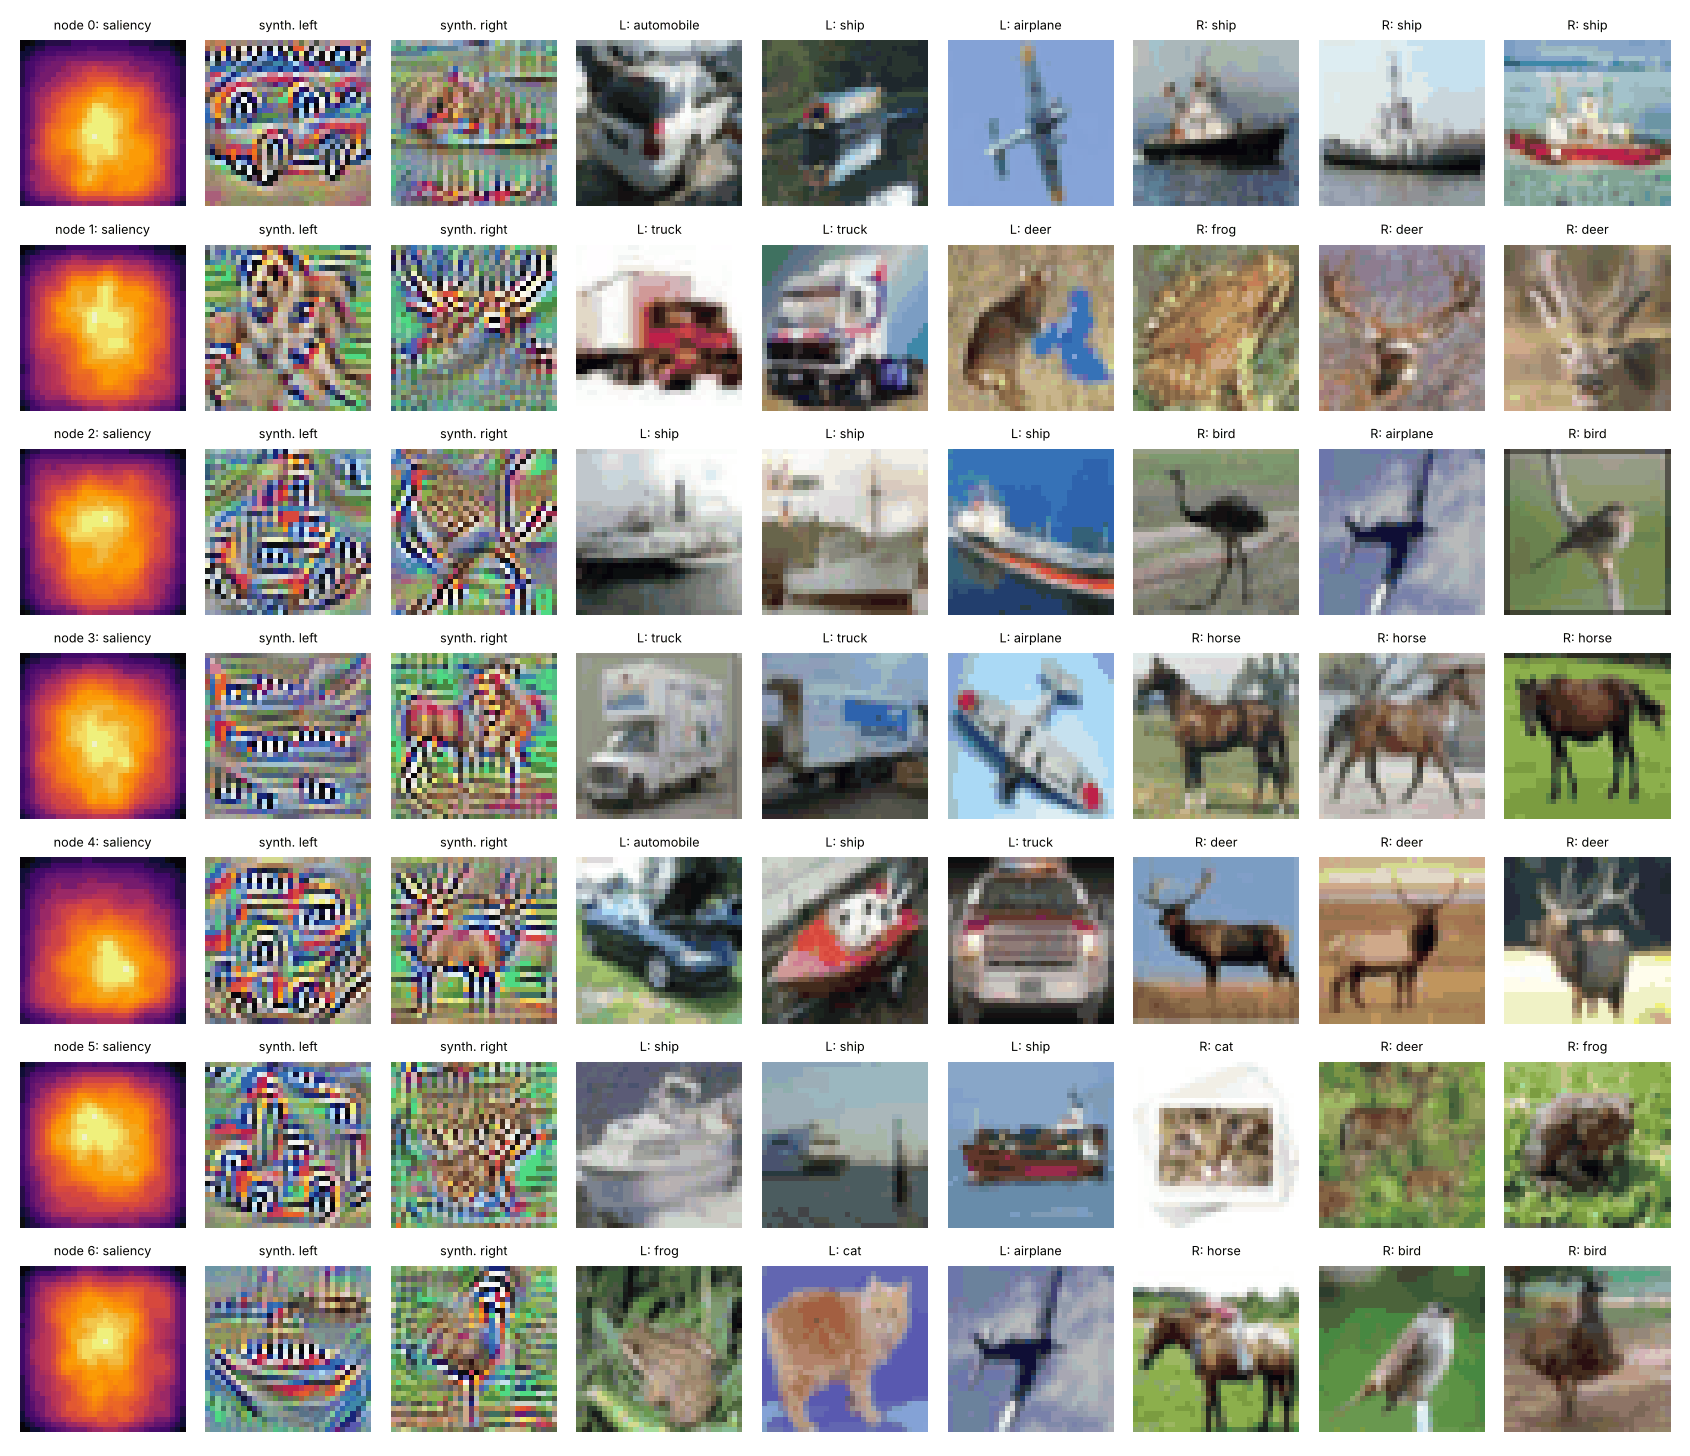
\includegraphics[width=\linewidth]{e3_routers_cifar10_cnn.png}
\caption{CIFAR-10, features from the CNN trained on CIFAR-10, same layout. Saliency now sits on the centre of the image, where the object is, and the synthesised images contain object parts: wheels and car bodies (node 0, left), antlers and legs (nodes 1 and 4, right), a horse (node 3, right), a bird (node 6, right). The root sends vehicles left.}
\label{fig:rf-c10-cnn}
\end{figure}

\begin{table}[t]
\centering\small
\begin{tabular}{llrrrrr}
\toprule
dataset & trunk & NMI(leaf, class) & NMI(root, vehicle) & mean router NMI & router radius & leaf radius \\
\midrule
CIFAR-10 & resnet & 0.225 & 0.044 & 0.125 & 0.74--0.76 & 0.74--0.75 \\
CIFAR-10 & cnn & 0.358 & 0.154 & 0.214 & 0.67--0.69 & 0.66--0.67 \\
Cats vs Dogs & resnet & 0.052 & -- & 0.057 & 0.71--0.74 & 0.71--0.74 \\
Cats vs Dogs & cnn & 0.145 & -- & 0.146 & 0.66--0.72 & 0.65--0.70 \\
\bottomrule
\end{tabular}

\caption{Receptive-field summary for the E1 trees. NMI(root, vehicle): agreement of the root decision with the animal/vehicle grouping. Radius: saliency-weighted distance from the centre (uniform map: 0.765).}
\label{tab:e3sum}
\end{table}

\begin{table}[t]
\centering\small
\begin{tabular}{rrlllr}
\toprule
node & images & left: top classes & right: top classes & NMI(split, class) & saliency radius \\
\midrule
0 & 10000 & frog, bird & truck, horse & 0.109 & 0.74 \\
1 & 5217 & frog, bird & cat, ship & 0.092 & 0.75 \\
2 & 4783 & truck, horse & dog, deer & 0.082 & 0.76 \\
3 & 3005 & frog, cat & frog, bird & 0.130 & 0.75 \\
4 & 2212 & cat, bird & ship, airplane & 0.152 & 0.76 \\
5 & 3047 & horse, truck & automobile, truck & 0.179 & 0.75 \\
6 & 1736 & deer, horse & dog, automobile & 0.134 & 0.75 \\
\bottomrule
\end{tabular}

\caption{CIFAR-10 routers, ResNet features.}
\label{tab:e3-c10}
\vspace{6pt}
\begin{tabular}{rrlllr}
\toprule
node & images & left: top classes & right: top classes & NMI(split, class) & saliency radius \\
\midrule
0 & 3000 & dog, cat & cat, dog & 0.003 & 0.74 \\
1 & 1672 & dog, cat & cat, dog & 0.030 & 0.73 \\
2 & 1328 & cat, dog & cat, dog & 0.001 & 0.72 \\
3 & 896 & dog, cat & dog, cat & 0.000 & 0.74 \\
4 & 776 & cat, dog & dog, cat & 0.149 & 0.72 \\
5 & 622 & dog, cat & cat, dog & 0.139 & 0.74 \\
6 & 706 & cat, dog & dog, cat & 0.076 & 0.71 \\
\bottomrule
\end{tabular}

\caption{Cats vs Dogs routers, ResNet features.}
\label{tab:e3-cd}
\end{table}

\paragraph{Observations.}
\begin{itemize}
\item \emph{On Cats vs Dogs the routers do not split by class.} With ResNet features the NMI between each router's decision and the label is between 0.000 and 0.15, and every leaf receives a mix of cats and dogs (NMI between leaf and class 0.05). The routers split by \emph{context}: wire fences and cages versus soft furnishings (node 1), dark versus light animals (node 0), whole body versus close-up face (node 2), grass and outdoors versus indoors (node 5). Each leaf then solves cat versus dog within one context, at 87--96\% test accuracy per leaf. With two classes there is little to route by class, and the balance penalty asks every router for an even split, so the routers follow the next strongest direction of variation in the features: background and photographic setting. These are the cues a classifier could use as shortcuts; here they decide which leaf sees the image rather than the label.
\item \emph{On CIFAR-10 the routers mix semantics and appearance.} With ResNet features the root does not separate animals from vehicles (NMI with that grouping 0.04); it sends frogs, birds and cats one way and trucks, horses and cars the other. The deepest routers are the most class-like (NMI 0.13 to 0.18, against 0.08 to 0.11 above them), and some splits group classes by background colour: node 4 puts ships and aeroplanes (sky and sea) together against birds in foliage.
\item \emph{The trunk decides what the nodes can see.} With the CNN trained on the task, routing is more semantic (leaf--class NMI 0.36 against 0.23 on CIFAR-10; root--vehicle NMI 0.15 against 0.04), saliency moves to the centre (radius 0.66--0.69 against 0.74--0.76) and the synthesised images show object parts instead of textures (Figure~\ref{fig:rf-c10-cnn}). The ImageNet trunk was never asked to find CIFAR objects, and at $64\times64$ its pooled features describe the whole scene; the task-trained trunk has learned to look at the centred object.
\item \emph{Depth in the tree does not shrink the receptive field.} For both trunks, radii of the root, the deeper routers and the leaves are within 0.07 of each other. The trunk ends in global average pooling, so every feature already depends on the whole image; nodes differ in \emph{what} they respond to (colour, texture, background, parts), not \emph{where}. This is unlike a CNN, where deeper units see larger regions: the tree's depth is a depth of decisions, not of spatial processing.
\item \emph{Pixel-tree routers memorise.} The router weights of the pixel tree (Figure~\ref{fig:pixel}) are mostly high-frequency noise; only the low-pass view shows structure (node 4 weights the border, nodes 2 and 5 a central blob). The pixel tree reaches 87\% training accuracy after 30 epochs but only 48\% test accuracy on CIFAR-10 (99\% and 65\% on Cats vs Dogs), which is why the main experiments use trunk features.
\end{itemize}

\begin{figure}[t]
\centering
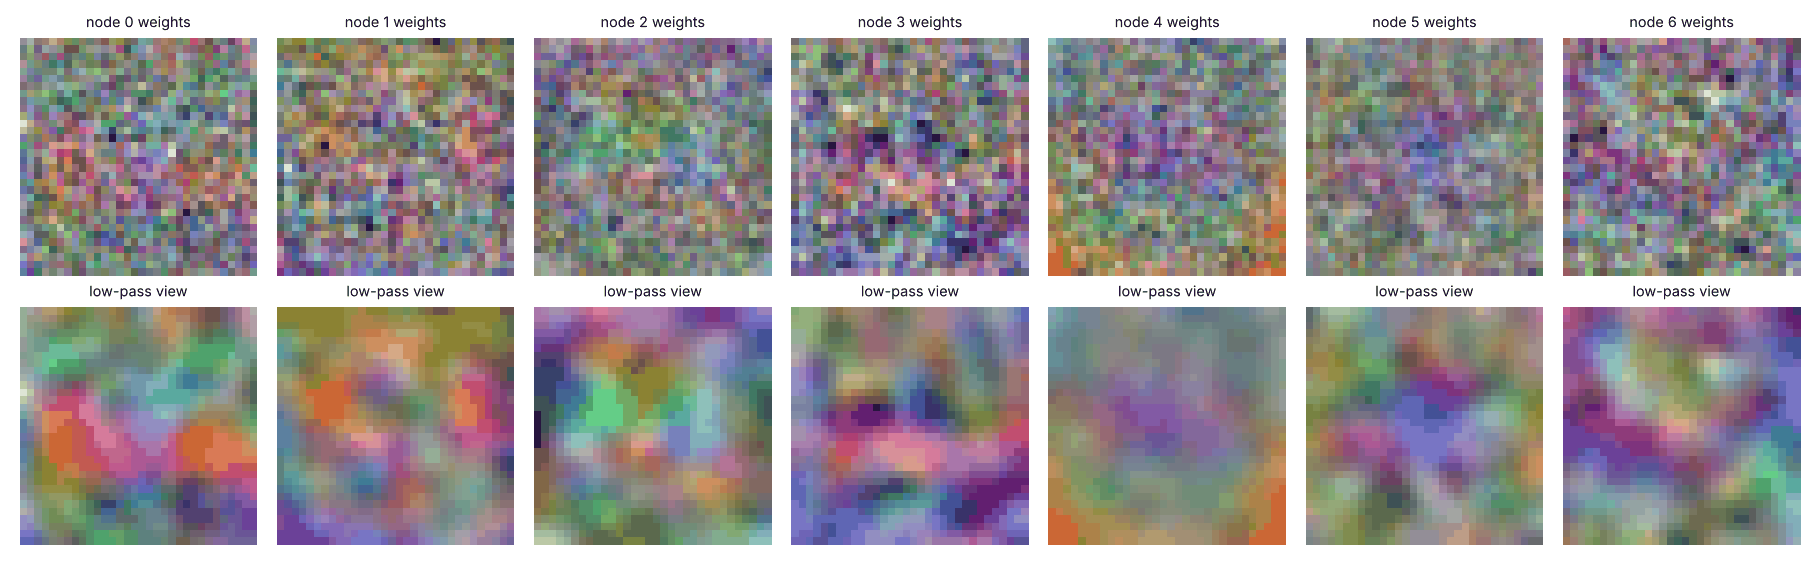
\includegraphics[width=\linewidth]{e3_pixeltree_cifar10.png}
\caption{Pixel tree on CIFAR-10: weights of the 7 linear routers (top) and the same weights after a Gaussian blur with $\sigma=1.5$ pixels (bottom). Each colour channel is scaled so that grey is zero.}
\label{fig:pixel}
\end{figure}

\section{E4: making the tree small}
\label{sec:e4}
Starting from the E1 trees on ResNet features (1.2M parameters), we tried six ways to shrink them (Table~\ref{tab:e4}, Figure~\ref{fig:e4}). All accuracies use hard routing.
\begin{description}
\item[Hard routing.] Only 3 routers and 1 leaf run per image: 217k of the 1.21M parameters, at a cost of 0.4 points on CIFAR-10 and none on Cats vs Dogs.
\item[Subtree collapse.] Greedily force one router to always pick one side (removing the other subtree) whenever this hurts validation accuracy least; repeat until one leaf remains. This is the neural version of cost-complexity pruning. On Cats vs Dogs the tree can be cut from 8 to 3 leaves with no loss (90.6\%); on CIFAR-10 accuracy falls step by step, to 80.4\% with 4 leaves and 78.7\% with 2.
\item[Magnitude pruning.] Remove the globally smallest weights, then fine-tune 3 epochs with the mask fixed, at increasing sparsity. At 90\% sparsity CIFAR-10 loses 1 point; at 99\% Cats vs Dogs still has 88.1\% with 13k stored and 2.8k per-image weights.
\item[Hidden-unit pruning.] Keep the $k$ strongest hidden units in each leaf. This is worse than unstructured pruning at equal size on both datasets.
\item[int8 weights.] Per-tensor 8-bit quantisation changes accuracy by less than 0.1 points and divides storage by 4.
\item[Small trees and distillation.] Train trees of 6 sizes from scratch, either on the labels or on the E1 tree's softened predictions (temperature 2).
\end{description}

\begin{table}[!htbp]
\centering\small
\begin{tabular}{lrrrrr}
\toprule
 & \multicolumn{2}{c}{CIFAR-10} & & \multicolumn{2}{c}{Cats vs Dogs} \\
\cmidrule{2-3}\cmidrule{5-6}
model & params & test acc & & params & test acc \\
\midrule
E1 tree, soft routing & 1210k & 82.5 & & 1202k & 90.6 \\
E1 tree, hard routing (per image) & 217k & 82.1 & & 216k & 90.6 \\
int8 weights (same count, 4x fewer bytes) & 1210k & 82.0 & & 1202k & 90.6 \\
magnitude pruned 90\%, stored & 122k & 81.0 & & 121k & 89.6 \\
magnitude pruned 90\%, per image & 25k & 81.0 & & 24k & 89.6 \\
magnitude pruned 99\%, stored & 13k & 73.9 & & 13k & 88.1 \\
magnitude pruned 99\%, per image & 2.6k & 73.9 & & 2.8k & 88.1 \\
subtree collapse, at most 3 leaves & 279k (2 leaves) & 78.7 & & 431k (3 leaves) & 90.6 \\
linear classifier, trained on labels & 9.6k & 82.3 & & 1.9k & 90.4 \\
linear classifier, distilled from E1 tree & 9.6k & 82.7 & & 1.9k & 90.9 \\
\bottomrule
\end{tabular}

\caption{E4 summary, ResNet features. ``per image'' counts weights on one root-to-leaf path.}
\label{tab:e4}
\end{table}

\begin{figure}[!htbp]
\centering
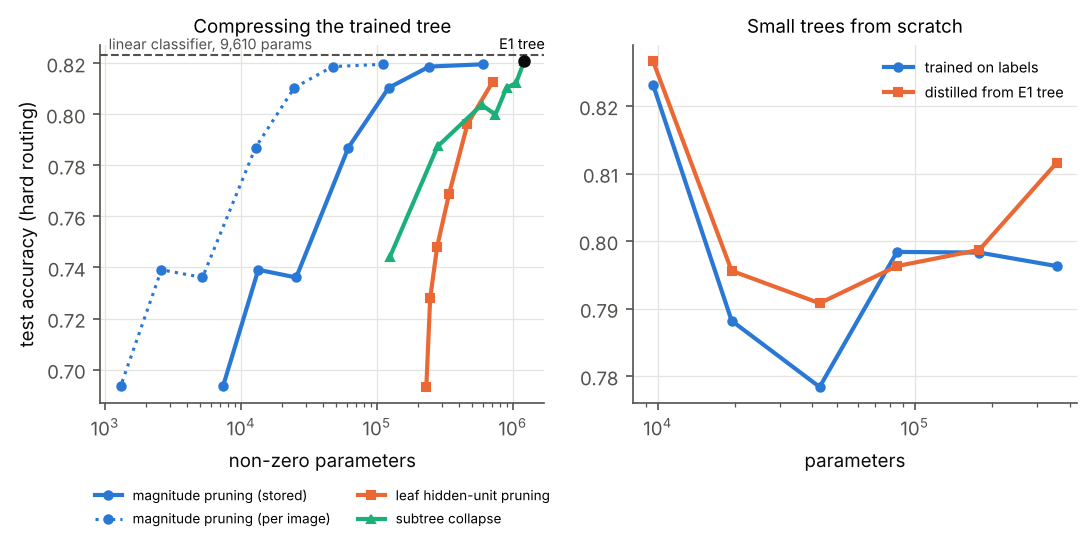
\includegraphics[width=\linewidth]{e4_cifar10.png}\\[2pt]
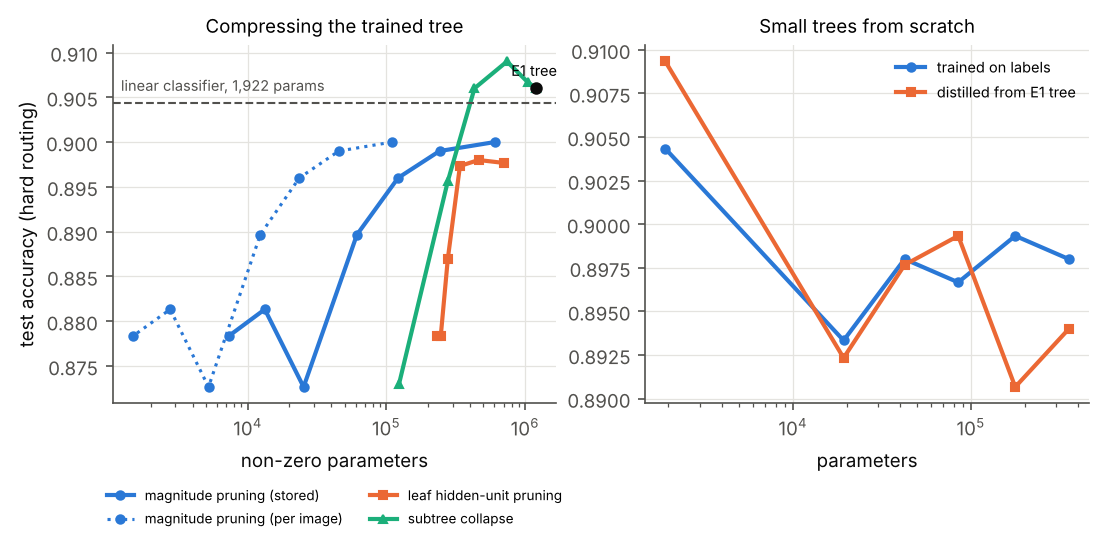
\includegraphics[width=\linewidth]{e4_catsdogs.png}
\caption{E4 on CIFAR-10 (top) and Cats vs Dogs (bottom). Left: compressing the E1 tree. Right: trees trained from scratch at each size; the leftmost point is a linear classifier (depth 0, no hidden layer).}
\label{fig:e4}
\end{figure}

The main result is the dashed line in Figure~\ref{fig:e4}: \textbf{a linear classifier on the same features, with 9.6k parameters on CIFAR-10 and 1.9k on Cats vs Dogs, is as accurate as the 1.2M-parameter tree} (82.3\% versus 82.5\%; 90.4\% versus 90.6\%), and a distilled linear classifier is slightly better than the tree it was distilled from (82.7\% and 90.9\%). The smallest network that matches the tree is therefore about 125 to 600 times smaller than it. The capacity of the big tree goes into memorising the training set, not into test accuracy.

The small trees trained from scratch (right panels) also show the smallest \emph{interpolating} tree. On CIFAR-10, a depth-2 tree with leaf width 16 (85k parameters) is the first to reach about 100\% training accuracy (99.95\%); smaller trees stop at 93.9\% and 98.2\%. Test accuracy goes from 82.3\% for the linear classifier down to 77.8\% at 43k parameters, where the tree can almost but not quite memorise the 45{,}000 images, and is back at 82.5\% for the 1.2M-parameter E1 tree. Cats vs Dogs shows the same dip, smaller (90.4\%, then 89.3\% at 19k, then 90.6\%). This is the double-descent shape on the full, clean training sets; Section~\ref{sec:dd} studies it under controlled conditions.
